% !TEX root = ../main.tex
\begin{figure}[htbp]
\centering
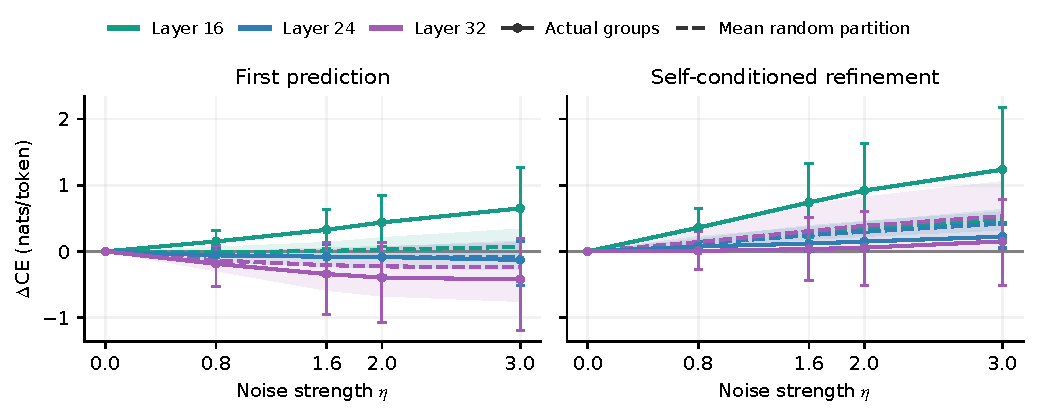
\includegraphics[width=\linewidth]{figures/layer_reconstruction_random.pdf}
\caption{\textbf{Layer groups expose distinct reconstruction sensitivities.} ELF-B epoch 18 on 64 GSM8K development problems. Solid curves perturb actual layer groups; dashed curves average eight random partitions with matched widths, times, and injected Gaussian energy. Colors identify the corresponding layer or control slot. Decoder CE changes are relative to the same pass's clean-input prediction: first without answer self-conditioning (left), then after one refinement on the same corrupted input (right). Error bars are pointwise 95\% problem-bootstrap intervals; shading is the range of random-partition means, not a confidence interval. Appendix~\ref{app:inferenceclocks} gives the intervention and paired contrasts.}
\label{fig:layerreconstruction}
\end{figure}
